\newpage
\section{Radial velocity with horizontal connection}

\subsection*{Resources}
\begin{itemize}
    \item Book sections 7/1 to 7/5
\end{itemize}

\emph{Correction to book: Figure 7/9 should read $\bm{\alpha} = \bm{\dot{\omega}} = \bm{\Omega} \bm{\times} \bm{\omega}$ (not $\bm{\Omega} \bm{\times} \bm{r}$)}

\subsection*{Challenge}
A weight ``A'' is tethered to a pole by a stiff rod of length $r$. If the angular velocity is \SI{5.5}{\radian\per\second} $\hat{k}$ and the length of the rod is \SI{47}{\meter} along the x-axis, what is the linear velocity of the weight ``A''?

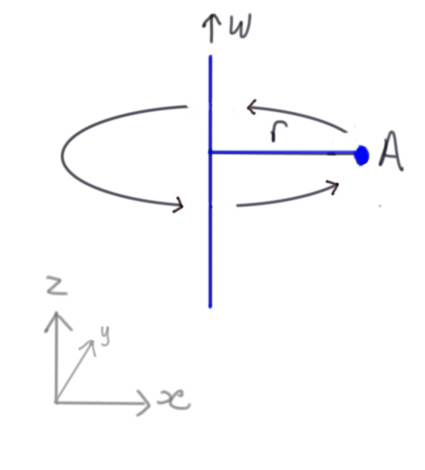
\includegraphics[height=5cm]{rod-horizontal}

\subsection*{Solution}
X = Your solution\\
Units: \si{\meter\per\second}\\
Form: Decimal, to 1 decimal place\\
Place the indicated letter in front of the number\\
Example: aX where $X=42.5$ \si{\meter\per\second} is entered as \href{http://www.wolframalpha.com/input/?i=md5+hash+of+\%22a42.5\%22}{a42.5}

$\hat{i}=$ hash of aX = 9497cd \si{\meter\per\second}\\
$\hat{j}=$ hash of bX = d17e5c \si{\meter\per\second}\\
$\hat{k}=$ hash of cX = 347133 \si{\meter\per\second}




\newpage
\section{Radial velocity with non-horizontal connection}

\subsection*{Resources}
\begin{itemize}
    \item Book sections 7/1 to 7/5
\end{itemize}

\emph{Correction to book: Figure 7/9 should read $\bm{\alpha} = \bm{\dot{\omega}} = \bm{\Omega} \bm{\times} \bm{\omega}$ (not $\bm{\Omega} \bm{\times} \bm{r}$)}

\subsection*{Challenge}
1. The position of ``A'' and the pole are unchanged (the radial distance is the same) and the angular velocity remains the same, but ``A'' is now hinged to the pole from below instead of horizontally, as shown in the picture. Calculate the linear velocity of ``A'' (calculate mathematically, not just by comparison with the previous challenge).

2. Write a sentence or two comparing your answer with that obtained from the previous challenge, including reasoning why.

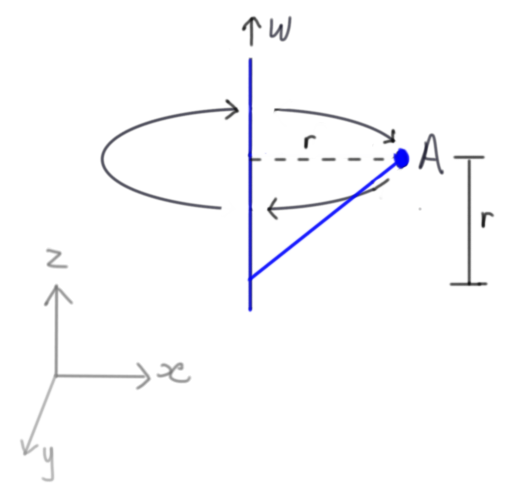
\includegraphics[height=5cm]{rod-frombelow}

\subsection*{Solution}
1.\\
X = Your solution\\
Units: \si{\meter\per\second}\\
Form: Decimal, to 1 decimal place\\
Place the indicated letter in front of the number\\
Example: aX where $X=42.5$ \si{\meter\per\second} is entered as \href{http://www.wolframalpha.com/input/?i=md5+hash+of+\%22a42.5\%22}{a42.5}

$\hat{i}=$ hash of dX = c6e675 \si{\meter\per\second}\\
$\hat{j}=$ hash of eX = bcff19 \si{\meter\per\second}\\
$\hat{k}=$ hash of fX = 979ed8 \si{\meter\per\second}

2. Please discuss in class if you are unsure about your answer.




\newpage
\section{Linear acceleration}

\subsection*{Resources}
\begin{itemize}
    \item Book sections 7/1 to 7/5
\end{itemize}

\emph{Correction to book: Figure 7/9 should read $\bm{\alpha} = \bm{\dot{\omega}} = \bm{\Omega} \bm{\times} \bm{\omega}$ (not $\bm{\Omega} \bm{\times} \bm{r}$)}

\subsection*{Challenge}
Using information from previous challenges, determine the:

1. Linear acceleration towards the centre of pole.

2. The tangential linear acceleration

3. Is there linear acceleration towards the centre of the pole? Is there tangential linear acceleration? Write a sentence or two to explain why for both cases.

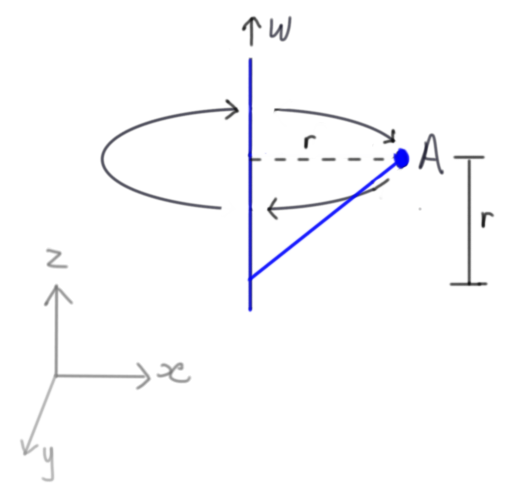
\includegraphics[height=5cm]{rod-frombelow}


\subsection*{Solution}
X = Your solution\\
Units: \si{\meter\per\square\second}\\
Form: Decimal, to 2 decimal place\\
Place the indicated letter in front of the number\\
Example: aX where $X=42.57$ \si{\meter\per\second} is entered as \href{http://www.wolframalpha.com/input/?i=md5+hash+of+\%22a42.5\%22}{a42.57}

1.\\
$\hat{i}=$ hash of gX = e1993f \si{\meter\per\square\second}\\
$\hat{j}=$ hash of hX = 5a16a7 \si{\meter\per\square\second}\\
$\hat{k}=$ hash of iX = 2ebd7c \si{\meter\per\square\second}

2.\\
$\hat{i}=$ hash of jX = 4b3090 \si{\meter\per\square\second}\\
$\hat{j}=$ hash of kX = 28435f \si{\meter\per\square\second}\\
$\hat{k}=$ hash of lX = 060ec3 \si{\meter\per\square\second}

3. Please compare your answer with your partner.




\newpage
\section{Radial acceleration - only magnitude}

\subsection*{Resources}
\begin{itemize}
    \item Book sections 7/1 to 7/5
\end{itemize}

\emph{Correction to book: Figure 7/9 should read $\bm{\alpha} = \bm{\dot{\omega}} = \bm{\Omega} \bm{\times} \bm{\omega}$ (not $\bm{\Omega} \bm{\times} \bm{r}$)}

\subsection*{Challenge}
Now consider that the radial velocity is not constant, but is undergoing an acceleration so that the magnitude of the angular velocity $\bm{w}$ increases while it continues to point in the same direction.

If the acceleration is \SI{2}{\radian\per\square\second}, what is the tangential acceleration of ``A''?

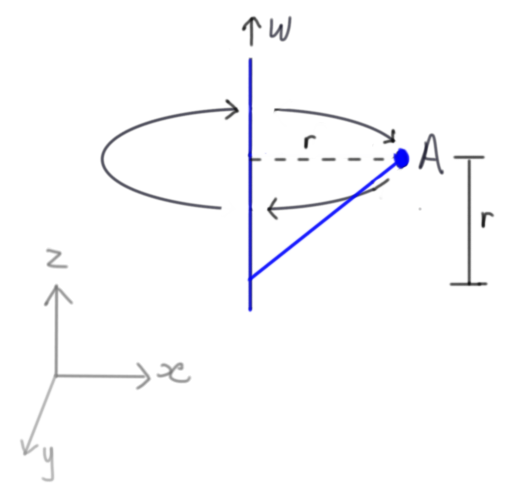
\includegraphics[height=5cm]{rod-frombelow}

\subsection*{Solution}
X = Your solution\\
Units: \si{\meter\per\second}\\
Form: Decimal, to 1 decimal place\\
Place the indicated letter in front of the number\\
Example: aX where $X=42.5$ \si{\meter\per\second} is entered as \href{http://www.wolframalpha.com/input/?i=md5+hash+of+\%22a42.5\%22}{a42.5}

$\hat{i}=$ hash of mX = b9f8f5 \si{\meter\per\second}\\
$\hat{j}=$ hash of nX = 57e394 \si{\meter\per\second}\\
$\hat{k}=$ hash of oX = 0c8b72 \si{\meter\per\second}





\newpage
\section{Radial acceleration - only direction (precession)}

\subsection*{Resources}
\begin{itemize}
    \item Book sections 7/1 to 7/5
\end{itemize}

\emph{Correction to book: Figure 7/9 should read $\bm{\alpha} = \bm{\dot{\omega}} = \bm{\Omega} \bm{\times} \bm{\omega}$ (not $\bm{\Omega} \bm{\times} \bm{r}$)}

\subsection*{Challenge}
The previous challenges considered the case (a) below, where the direction of the angular velocity vector $\omega$ was unchanging. Next consider that the angular velocity vector is precessing around an axis of symettry, and this precession has an angular velocity of $\Omega$, as shown in (b). Combining (a) and (b) we have (c).

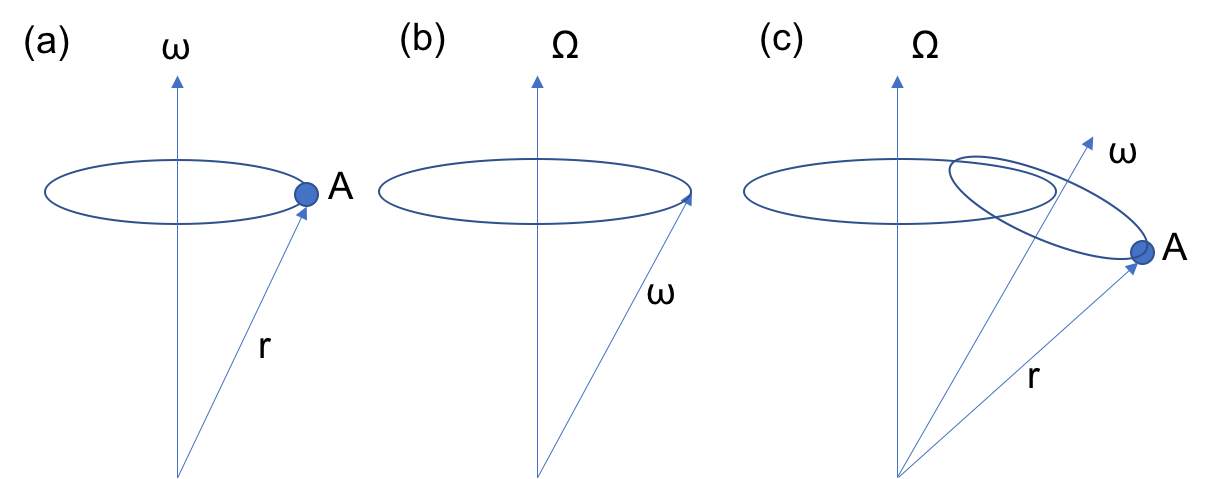
\includegraphics[height=5cm]{precession}

1. Consider the same system as before, but tilt the $\omega$ vector and allow the rotation to precess around a vector of symmetry $\Omega$. Assuming that only the direction (not the magnitude) of the angular velocity vector $\omega$ is changing with time, calculate the linear acceleration of ``A'' if $\Omega = 3\hat{k}$ \si{\radian\per\second} and angular velocity vector $\omega$ is inclined at \SI{45}{\degree} with components $\omega = 5.5 \hat{i} + 5.5 \hat{k}$. You may assume all other properties are the same as recent previous challenges.

2. What is the direction of the acceleration of the angular velocity vector $\omega$. Write 1 or 2 sentences to explain why.

3. What is the direction of the linear acceleration of ``A''. Write one or two sentences (possibly with a diagram) to explain when the sign will be opposite but with same magnitude.


\subsection*{Solution}
1. $-873 \hat{i} + 873 \hat{k}$

2. and 3. Please discuss in class.




\newpage
\section{Radial acceleration II}

\subsection*{Resources}
\begin{itemize}
    \item Book sections 7/1 to 7/5
\end{itemize}

\emph{Correction to book: Figure 7/9 should read $\bm{\alpha} = \bm{\dot{\omega}} = \bm{\Omega} \bm{\times} \bm{\omega}$ (not $\bm{\Omega} \bm{\times} \bm{r}$)}

\subsection*{Challenge}
Question 7/4

\subsection*{Solution}
\SI{1285}{\meter\per\second}




\newpage
\section{Unit vector of a rotation axis}

\subsection*{Resources}
\begin{itemize}
    \item Book sections 7/1 to 7/5
\end{itemize}

\emph{Correction to book: Figure 7/9 should read $\bm{\alpha} = \bm{\dot{\omega}} = \bm{\Omega} \bm{\times} \bm{\omega}$ (not $\bm{\Omega} \bm{\times} \bm{r}$)}

\subsection*{Challenge}
Considering vector $\bm{r}$ in the figure below, if the angles $\alpha = 45$ degrees and $\beta = 30$ degrees, write the unit vector $\bm{\hat{r}}$ in terms fo the cartesian unit vectors.

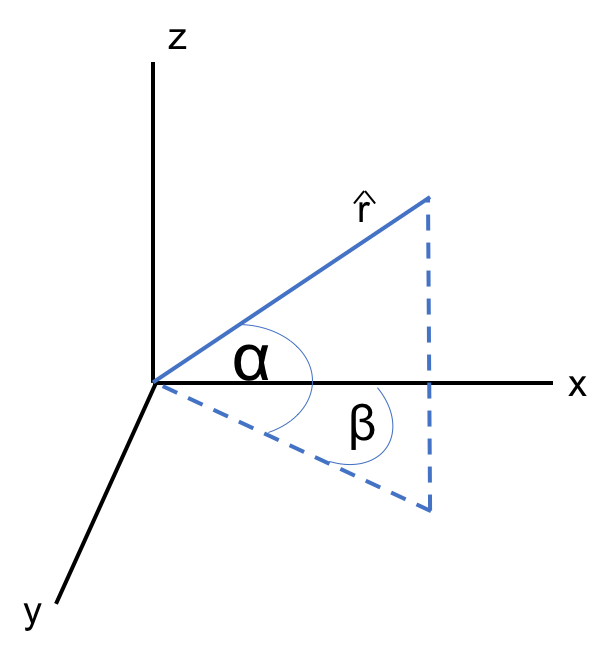
\includegraphics[height=5cm]{angles_vectors}

\subsection*{Solution}
$\bm{r} = \frac{1}{\sqrt{2}} \hat{i} + \frac{1}{\sqrt{6}} \hat{j} + \frac{1}{\sqrt{3}} \hat{k}$


\newpage
\section{Simultanious rotation I}

\subsection*{Resources}
\begin{itemize}
    \item Book sections 7/1 to 7/5
\end{itemize}

\emph{Correction to book: Figure 7/9 should read $\bm{\alpha} = \bm{\dot{\omega}} = \bm{\Omega} \bm{\times} \bm{\omega}$ (not $\bm{\Omega} \bm{\times} \bm{r}$)}

\subsection*{Challenge}
Work through sample problem 7/2.




\newpage
\section{Simultanious rotation II}

\subsection*{Resources}
\begin{itemize}
    \item Book sections 7/1 to 7/5
\end{itemize}

\emph{Correction to book: Figure 7/9 should read $\bm{\alpha} = \bm{\dot{\omega}} = \bm{\Omega} \bm{\times} \bm{\omega}$ (not $\bm{\Omega} \bm{\times} \bm{r}$)}

\subsection*{Challenge}
Work through sample problem 7/1, parts (a) and (b) only.




\newpage
\section{Simultanious rotation III}

\subsection*{Resources}
\begin{itemize}
    \item Book sections 7/1 to 7/5
\end{itemize}

\emph{Correction to book: Figure 7/9 should read $\bm{\alpha} = \bm{\dot{\omega}} = \bm{\Omega} \bm{\times} \bm{\omega}$ (not $\bm{\Omega} \bm{\times} \bm{r}$)}

\subsection*{Challenge}
Complete question 7/12


\subsection*{Solution}
$\frac{-\pi^2}{8}(25 \hat{j} + 18 \hat{k})$ \si{\meter\per\second}




\newpage
\section{Time-dependent rotation of vectors I}

\subsection*{Comment}
A vector $\bm{r}$ may be split into its magnitude and scaler components like $\bm{r} = r_i \bm{\hat{i}} + r_j \bm{\hat{j}} + r_k \bm{\hat{k}}$. For fixed co-ordinate systems, the direction of ($\bm{\hat{i}}$, $\bm{\hat{j}}$, $\bm{\hat{k}}$) does not vary with time, so the derivatives of the unit vectors are zero. For a rotating co-ordinate system however, the derivative chain rule must be used in order to take account of the changing directions of the unit vectors.

\subsection*{Challenge}
Consider a disk that is initially flat in the x-y plane. The z-axis can be considered to point perpendicularly up from the centre of the disk. The disk then starts spinning with angular velocity depending on time $t$:
\begin{equation}
    \bm{\omega} = \omega_i Sin(2 \pi t) \bm{\hat{i}} + \omega_j Cos(2 \pi t) \bm{\hat{j}} + \omega_k t \bm{\hat{k}}
\end{equation}

You can consider the $\bm{\hat{i}}$ and $\bm{\hat{j}}$ axes to be rotating with the disk and the $\bm{\hat{k}}$ vector to always point perpendicular to the plane of the disk. 

Derive an expression for the angular acceleration $\bm{\dot{\omega}}$ of the disk as a function of time.


\subsection*{Solution}
To check your answer, substitute the following values into your final equation:
$t=1$\\
$\omega_i=10$
$\omega_j=3$
$\omega_k=2$

and you should obtain the final result

$\bm{\dot{\omega}} = (20 \pi - 6) \bm{\hat{i}} + 2 \bm{\hat{k}}$




\newpage
\section{Time-dependent rotation of vectors II}

\subsection*{Challenge}
Answer question 7/27 in the book.

\subsection*{Solution}
Given in book.
